\chapter{Аналіз ефективності нейромережевих методів для генерації синтетичних текстів}

%%%%%%%%%%%%%%%%%%%%%%%%%%%%%%%%%%%%%%%%%%%%%%%%%%%%%%%
\section{Дослідження впливу математичних розділів задач на ефективність генерації розв'язків}

Цей підрозділ представляє статистичний аналіз ефективності розв’язання задач у різних математичних розділах на протестованих моделях. Як згадувалося раніше задачі були розподілені 4 основні математичні розділи: алгебра, комбінаторика, геометрія та теорія чисел.

Для проведення результати спочатку було отримано середню частоту правильних розв'язків моделей за різними розділами. Далі було використано статистичний критерій хі-квадрат та метод перестановок для оцінки того, чи є розподіл правильних та неправильних розв'язків між розділами статистично значущим, а також для визначення середніх показників ефективності протестованих моделей до кожного окремо розглянутого математичного розділу.

\begin{figure}[!h]
    \centering
    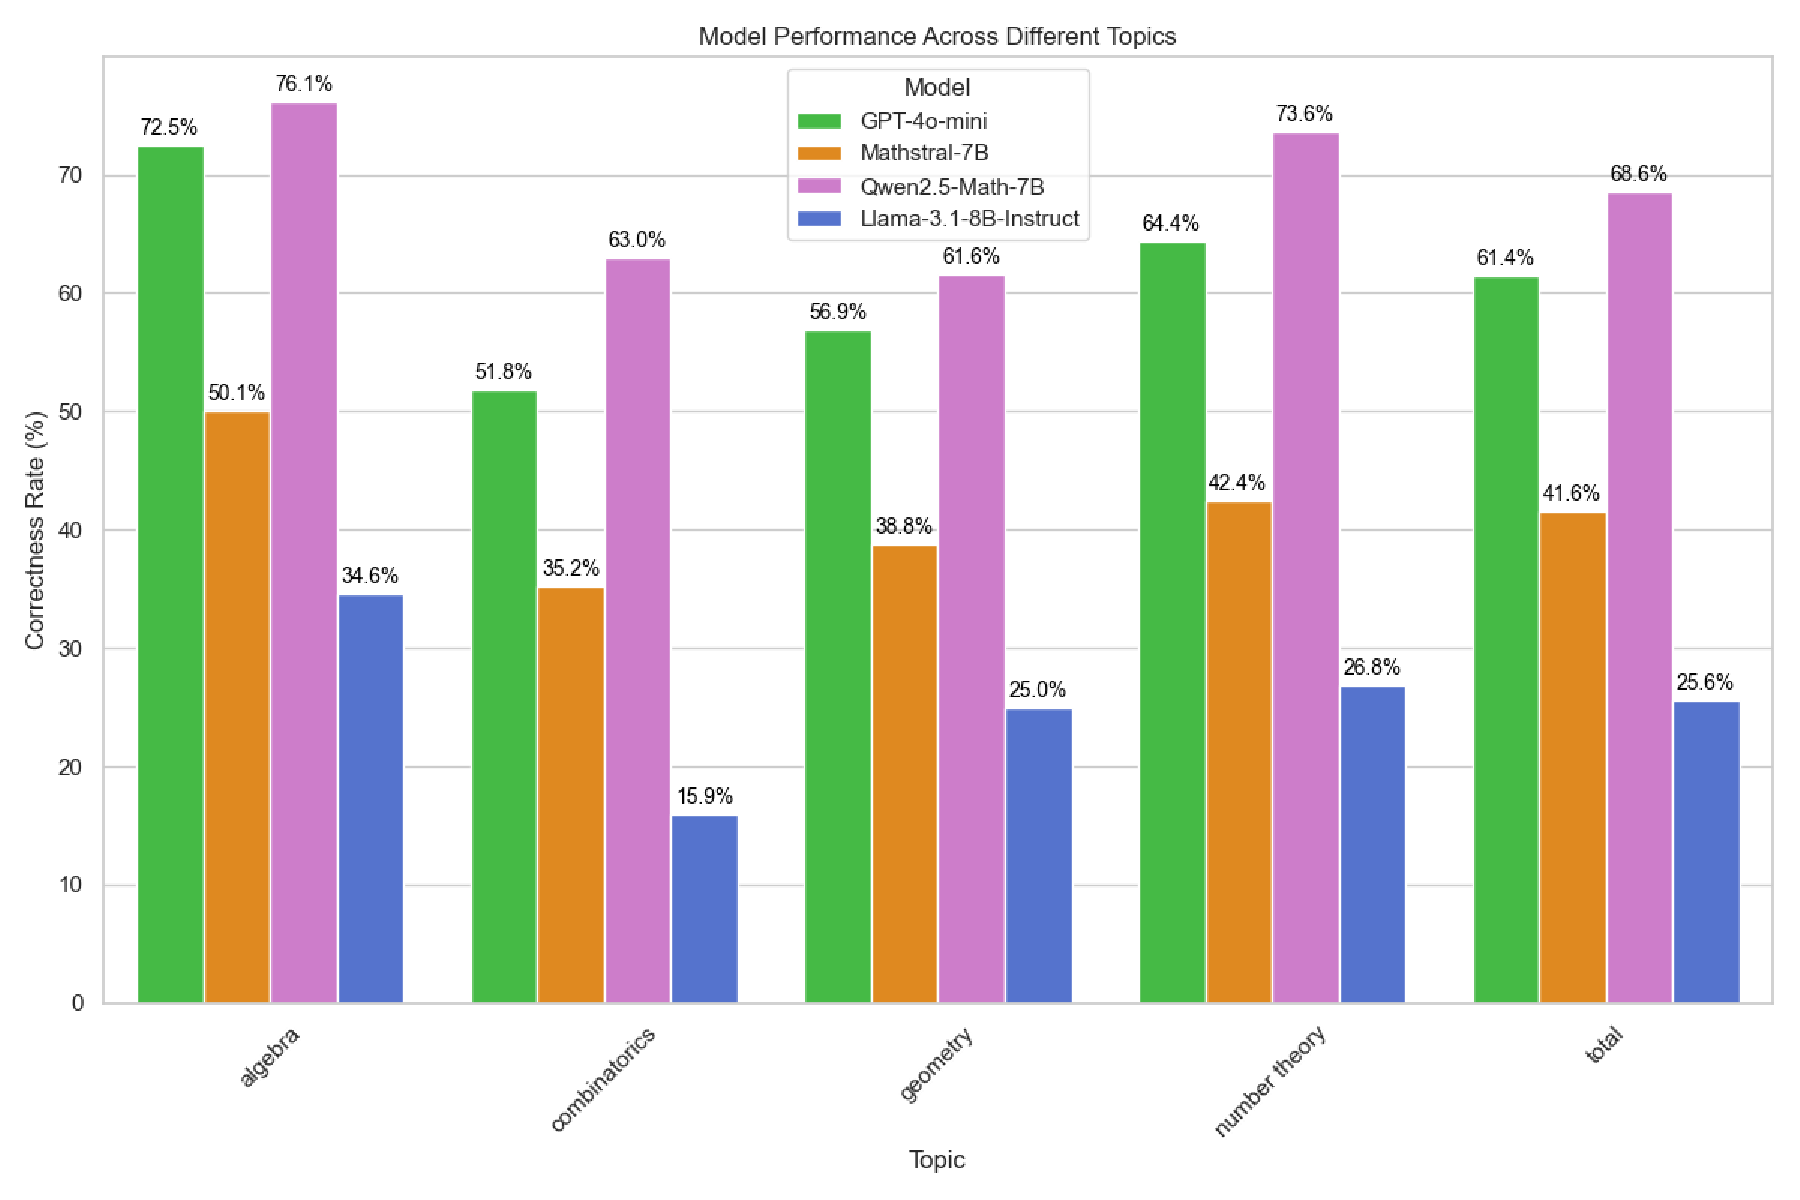
\includegraphics[width=0.9\textwidth]{correctness_rate.pdf}
    \caption{Середня точність розв'язків по різних математичних розділах моделями GPT-4o-mini (зелений), Mathstral-7B (помаранчевий), Qwen2.5-Math-7B (фіолетовий), Llama-3.1-8B-Instruct (блакитний).}
    \label{fig:correctness_rate}
\end{figure}

Загальні результати показали, що моделі досягають найкращих результатів 
з задачами у алгебраїчному розділі, тоді як комбінаторика виявилася найскладнішим розділом. З рисунку~\ref{fig:correctness_rate}) можна бачити, що частота правильних розв'язків згенерованих моделями склала між 34.6-76.1\% в алгебрі, тоді як у комбінаториці результати становили між 15.9-63.0\%.

\subsection{Ефективність моделей у розв'язанні задач з алгебри, геометрії, теорії чисел та комбінаторики}

Було обчислено середній рівень точності моделей для кожного математичного розділу у вигляді відсотку правильних розв'язків. Дані результати надають уявлення про загальну ефективність моделей у розв'язанні математичних задач та їхню чутливість до відповідних типів задач.

З рис.~\ref{fig:correctness_rate} видно, що мовна модель Qwen2.5-Math-7B продемонструвала найкращу середню частоту правильних розв'язків -- 68.6\%, тоді як модель Llama-3.1-8B-Instruct показала найгірші результати –- 25.6\%.

Із Таблиці~\ref{tab:p_values} спостерігається, що найвищі середні показники ефективності моделей за розділами (Average Mathematical Performance in Domain, AMPD) були досягнуті в алгебрі $AMPD_{algebra} = 58\%$, що свідчить про найбільшу точність роботи моделей у відповідному розділі. У розділі теорії чисел результат досягнув $AMPD_{number\space theory} = 58\%$, показуючи відносно високі результати. Геометрія та Комбінаторика мають нижчі AMPD: $AMPD_{geometry} = 46\%$ та $AMPD_{combinatorics} = 41\%$, що вказує на більшу більшу складність відповідних розділів для розв'язання моделями. Таблиця також свідчить про те, що всі спостережувані відмінності є статистично значущими -- про ще описано детальніше у наступному розділі~\fullref{sec:ampd-stats}.

\begin{figure}[!h]
\centering \small
    \captionof{table}{Різниця ефективності роботи моделей між усередненими результатами моделей за математичними розділами. ``*'' означає, що різниця в розділі була дуже значущою ($p < 0.001$).}
    \label{tab:p_values}
    \begin{tabular}{|l|c|cccc|}
    \hline
    розділ & & алгебра & комбінаторика & геометрія & теорія чисел \\
    \hline
    & AMPD & 0.58 & 0.41 & 0.46 & 0.52 \\
    \hline
    алгебра & 0.58 & – &  &  &  \\
    комбінаторика & 0.41 & \textbf{0.17*} & – &  &  \\
    геометрія & 0.46 & \textbf{0.13*} & \textbf{0.04*} & – &  \\
    теорія чисел & 0.52 & \textbf{0.07*} & \textbf{0.10*} & \textbf{0.06*} & – \\
    \hline
    \end{tabular}
\end{figure}

\begin{itemize}
    \item {Алгебра}. Найвищий для моделей частота розв'язання задач була досягнута за алгебраїчною тематикою: GPT-4o-mini досягла правильності у 72.5\%, а Qwen2.5-Math-7B –- 76.1\%. Ці показники вказують на високий рівень стійкості роботи з алгебраїчними задачами, ймовірно за рахунок більш явного подання задач у формальному вигляді, що спрощує пошук відповідних методів до розв'язання задач та символьної обробки текстів.
    
    \item {Комбінаторика}. Комбінаторні задачі показували суттєво гірші результати на більшості моделей. Модель Mathstral-7B мала значні труднощі з генерацією правильних розв'язків (отримано лише 35.2\% правильних розв'язків), GPT-4o-mini також показала не найкращі результати з відповідними задачами (51.8\%). Скоріше за все це обумовлено незвичністю комбінаторного стилю задач, який мають більш природній а не формальний вигляд відповідних текстів задач.
    
    \item {Геометрія}. У геометрії модель Mathstral-7B досягла частоти правильних розв'язків рівний 38.8\%, що свідчить про поганий рівень володіння даною темою. Натомість GPT-4o-mini і Qwen2.5-Math-7B були більш успішними та досягли 56.9\% та 61.6\% частоти правильних розв'язків, тим самим демонструючи відносно гарні результати роботи.
    
    \item {Теорія чисел}. У задачах за темою теорії чисел були отримані змішані результати. Для моделі Mathstral-7B частота правильності надання розв'язків склала 42.4\%, що вказує на певні труднощі з темою. Проте Qwen2.5-Math-7B продемонстрували суттєво кращий рівень володіння темою, досягнувши 73.6\%.
\end{itemize}

\subsection{Статистична значущість отриманих результатів}
\label{sec:ampd-stats}

\paragraph{Результати аналізу тесту критерію хі-квадрат}
Було проведено тест значущості отриманих результатів за критерієм хі-квадрат задля того, щоб оцінити, чи впливає математичний розділ на розподіл правильних та неправильних розв'язків. Відповідні значення наведені у Таблиці~\ref{tab:chi_square_results}. Усі досліджені моделі мають ступені свободи $D_{f} = 3$ (кількість розглянутих розділів мінус 1), а значення $p\text{-}value$ було значно нижчим за 0.05.

\begin{figure}[!h]
    \centering
    \captionof{table}{Результати тесту критерію хі-квадрат для кожної моделі та комбіноване значення.}
    \label{tab:chi_square_results}
    \begin{tabular}{|l|l|}
    \hline
    Модель & Хі-квадрат \\
    \hline
    GPT-4o-mini & 205.64 \\
    Mathstral-7B & 101.04 \\
    Qwen2.5-Math-7B & 149.37 \\
    Llama-3.1-8B-Instruct & 184.93 \\
    \hline
    Комбіноване значення & 520.16 \\
    \hline
    \end{tabular}
\end{figure}

З Таблиці~\ref{tab:chi_square_results} видно, що міру комбінованого значення, що підкреслює загальний вплив математичних розділів на ефективність роботи моделей. Високе середнє значення $\chi^2=520.16$ свідчить про те, що розділ є суттєвою характеристикою на роботу моделей, що підтверджує наявність різниці в результатах частоти надання правильних розв'язків в залежності від обраного математичного розділу.

Найвищий рівень хі-квадрат має модель GPT-4o-mini ($\chi^2_{\text{GPT-4o-mini}}=205.64$). Даний результат вказує на те, що для моделі існує висока залежність між математичними розділами задач та точністю роботи моделі у генерації розв'язків. Інакше кажучи в залежності від теми отриманої на вхід задач, модель має суттєво різні шанси на її отримання правильного розв'язання.

Зі значенням $\chi^2_{\text{Mathstral-7B}}=101.04$ модель Mathstral-7B показує найменшу чутливість до розділу в генерації правильних розв’язків. Хоча вплив розділу все ще є суттєвим, він є менш вираженим у порівнянні з іншими моделями.

Загалом, результати підкреслюють те, що всі моделі відчувають суттєвий рівень впливу математичного розділу задач, з особливо суттєвою чутливістю у роботі моделей GPT-4o-mini та Llama-3.1-8B-Instruct.

\paragraph{Результати аналізу тесту перестановок}
Для подальшого аналізу впливу математичних розділів на роботу моделей було проведено тест перестановок. Як можна бачити з Таблиці~\ref{tab:p_values}, тест перестановок незмінно повертав значення $p\text{-}value < 0.001$ за усіма математичними розділами, тим самим підтверджуючи отримані результати критерію хі-квадрат.

Таким чином, статистичний аналіз вказує на суттєві відмінності в ефективності роботи ВММ в залежності від залежності вхідних задач та досліджуваних математичних розділів. Результати вказують на те, що ймовірність генерації правильного розв'язку задачі залежить від її належності до розділу алгебри, комбінаторики, геометрії або теорії чисел.

Додатково слід зазначити, що однією з причин впливу на значущість різниці у результатах роботи моделей є особливості налаштування обробки отриманих результатів за допомогою регулярних виразів для вилучення розв'язків, які також впливають на отримання відповідних значень роботи моделей.

Під час проведення експериментів найнижчий рівень ефективності досліджуваних моделей було зафіксовано у комбінаториці, а найвищий –- в алгебрі. Дані результати у загальному розумінні свідчать про те, що для мовних моделей ефективність генерації розв'язань на тему комбінаторики є найнижчою, тим самим роблячи даний розділ найбільш цікавим з точку зору подальшого дослідження. Таким чином, це підтверджує необхідність вибору та зосередження уваги у даній дисертаційній роботі на математичних комбінаторних задачах.

%%%%%%%%%%%%%%%%%%%%%%%%%%%%%%%%%%%%%%%%%%%%%%%%%%%%%%%
\section{Дослідження впливу варіацій комбінаторних задач на ефективність моделей}

\subsection{Порівняння великих мовних моделей на наборі даних Combi-Puzzles} 
Для подальшого проведення аналізу на математичних комбінаторних задачах перейдемо до результатів експерименту у порівнянні можливостей міркування розглянутих у відповідному експерименті ВММ. У Таблиці~\ref{tab:best_model} наведено показники кожної моделі у різних варіаціях, з/без додаткових інструкцій, та загальні результати. З Таблиці~\ref{tab:best_model} можна спостерігати, що GPT-4 показав найкращі результати у всіх формах задач, незалежно від стратегії задання запитів задач. Найкращий середній загальний результат отримано при постановці питань до GPT-4 без додаткових інструкцій (загальний бал 78\%). Значних відмінностей між стратегіями інструкції виявлено не було, проте через те, що різниця у ефективності роботи моделей у середньому є кращою для запитів без додаткових інструкцій, подальший аналіз було зосереджено на відповідних результатах.

\begin{figure}[!h]
    \centering 
    \small 
    \captionof{table}{Середні значення ефективності моделей на варіаціях математичних комбінаторних задач та загальні результати для двох стратегій: із додатковою інструкцією ``Короткий та правильний розв'язок'' (``The short and correct answer is'') (знизу) і без додаткової інструкції (зверху).} 
    \label{tab:best_model} 
    \begin{tabular}{|l|ccccc|c|}
    \hline
    Модель & Комб. & Мат. & Надлишк. & Парам. & Лінг. & Загальний \\
    \hline
    GPT-4 & \textbf{.82} & \textbf{.94} & \textbf{.77} & \textbf{.67} & \textbf{.70} & \textbf{.78} \\
    LLaMA-2 &.22 & .22 & .15 & .19 & .11 & .18 \\
    LLaMA-3.1 & .54 & .60 & .50 & .42 & .48 & .51 \\
    Mixtral & .42 & .38 & .26 & .23 & .23 & .30 \\
    \hline
    GPT-4 &  .76 & .90 & .76 & .61 & .66 & .74 \\
    LLaMA-2 & .19 & .17 & .05 & .08 & .11 & .12 \\
    LLaMA-3.1 & .53 & .61 & .43 & .40 & .52 & .50 \\
    Mixtral & .41 & .34 & .18 & .30 & .22 & .29 \\
    \hline
    \end{tabular}
\end{figure}

\subsection{Дослідження рівню впливу варіацій задач на роботу великих мовних моделей}
Аналіз показав, що моделі демонструють високу ефективність у математичній варіації задач, на яких модель GPT-4 досягла 94\%, проте ефективність моделей суттєво знижується при введенні додаткових лінгвістично-стилістичних маніпуляцій, які модифікують умови задач (варіації: надлишкова, параметризована та лінгвістичне заплутування).

\begin{figure}[!h]
    \centering
    \small
    \captionof{table}{Порівняння відмінностей між варіаціями для результатів GPT-4 у різних варіаціях. '*' означає, що різниця між варіаціями була значущою ($p < .05$).}
    \label{tab:forms_diff}
    \begin{tabular}{|l|c|ccccc|}
    \hline
    & & Звич. & Мат. & Надл. & Парам. & Лінг. \\
    \hline
    Модель GPT-4 & & .82 & .94 & .77 & .67 & .70 \\
    \hline
    Звичайна & .82 & - &  &  &  &  \\
    Математична & .94 & .12 & - &  &  &  \\
    Надлишкова & .77 & -.05 & \textbf{-.17*} (.026) & - &  &  \\
    Параметризована & .67 & -.15 & \textbf{-.27*} (.002) & -.10 & - &  \\
    Лінгвістичне заплутування & .70 & -.12 & \textbf{-.24*} (.006) & -.07 & .03 & - \\
    \hline
    \end{tabular}
\end{figure}

\paragraph{Ефективність роботи моделей у розв'язанні задач зі зайвою інформацією}
Моделі зазнають зниження точності при внесенні надлишкової інформації або лінгвістичного шуму в умови задач, але при цьому зберігають достатній рівень точності у відповідних варіаціях задач. У випадку варіацій з надлишковою інформацією, яка включає додавання зайвої числової інформації, GPT-4 отримав вищий бал -- 77\%, у той час як експерти -- 64\%, проте ця різниця не є статистично значущою ($p=.185$). Це свідчить про те, що порівняно з мовними моделями люди можуть сильніше піддаватися впливу зайвої інформації у коротких задачах (з меншою довжиною вхідного тексту) \cite{nikolaiev2024can}.

\paragraph{Ефективність роботи моделей у розв'язанні задач із лінгвістично-стилістичними модифікаціями}
Лінгвістично-стилістичні маніпуляції з текстами задач, такі як зміна стилю чи додавання нерелевантних деталей, впливають на ефективність роботи моделей. Для варіації лінгвістичного заплутування, різниця між моделями та людьми є менш значною (70\% для моделей та 74\% для людей), і у середньому дещо кращою для людей, однак дана різниця не є статистично значущою ($p=.714$). На відмінність від задач з зайвою інформацією даний результати говорить про те, що моделі гірні відокремлюють релевантну інформації у довших задач (з більшою середньою довжиною текстів). 

\paragraph{Ефективність роботи моделей у розв'язанні задач зі зміною конфігурації}
Моделі стикаються з труднощами при розв'язанні задач з більшими конфігураціями. У параметризованій варіації задач, ефективність GPT-4 (67\%) порівняно з експертами (70\%) є майже однаковою, що вказує на гіршу точність роботи моделей при обробці більш складних обчислень.

\paragraph{Ефективність роботи моделей у розв'язанні задач із додатковими обмеженнями}
Для оцінювання ефективності мовних моделей у роботі з додатковими обмеженнями їм подавали комбінаторну задачу у текстовому вигляді. Умова задачі формулювалася у двох варіантах: без обмежень та з додатковими обмеженнями.
Результати експерименту виявили обмеження мовних моделей у побудові міркувань при розв’язанні задач з додатковими умовами. Зокрема збільшення моделі не завжди призводить до підвищення їхньої ефективності при роботі з даними задачами. Водночас людина здатна гнучко обробляти суттєві елементи задачі, які впливають на пошук відповіді.
Генеративні моделі, які не мають спеціальних механізмів міркування, демонструють труднощі в інтерпретації модифікованих версій задач, що призводить до некоректного пошуку розв’язку. Це вказує на важливість інтеграції внутрішніх стратегій міркування та прийняття рішень у мовних моделях.


%%%%%%%%%%%%%%%%%%%%%%%%%%%%%%%%%%%%%%%%%%%%%%%%%%%%%%%
\section{Аналіз згенерованих варіацій задач}

\subsection{Статистичні вимірювання}

Для оцінки статистичної значущості відмінностей між варіаціями задач було використано пермутаційний тест (permutation test). Даний тест було обрано через його здатність оцінювати нульову гіпотезу без вимог до нормальності розподілу, також даний тест є надійний при роботі з невеликими обсягами даних. Даний тест було проведено задля того, щоб порівняти правильність відповідей у стовпчиках \texttt{original\_ans}, \texttt{fictional\_ans}, \texttt{adversarial\_ans} та \texttt{contdis\_ans} розв'язку та вилучення відповідей, отриманих за допомогою методу, зі стовпчиком \texttt{answer}, яка є базовою відповіддю. Кожне порівняння зі стовпчиком \texttt{answer} дозволяє визначити, чи є відхилення, що спостерігаються у варіаціях, статистично значущими. Результати роботи відображено на рисунку \ref{fig:versions}, тоді як тест на значущість -- у таблиці~\ref{tab:sign_test}.

\begin{figure}[ht]
    \centering
    \captionof{table}{Порівняння розв'язаних варіацій з очікуваною відповіддю заданих у p-значеннях. `*' вказує на те, що різниця в значеннях варіацій була значущою ($p < .05$).}
    \label{tab:sign_test}
    \begin{tabular}{|c|c|c|c|}
    \hline
    Оригінальна & Художня & Надлишкова & Прихована \\
    \hline
    .247 & .494 & \textbf{.029*} & .244 \\
    \hline
    \end{tabular}
\end{figure}

\begin{figure}[ht]
    \centering
    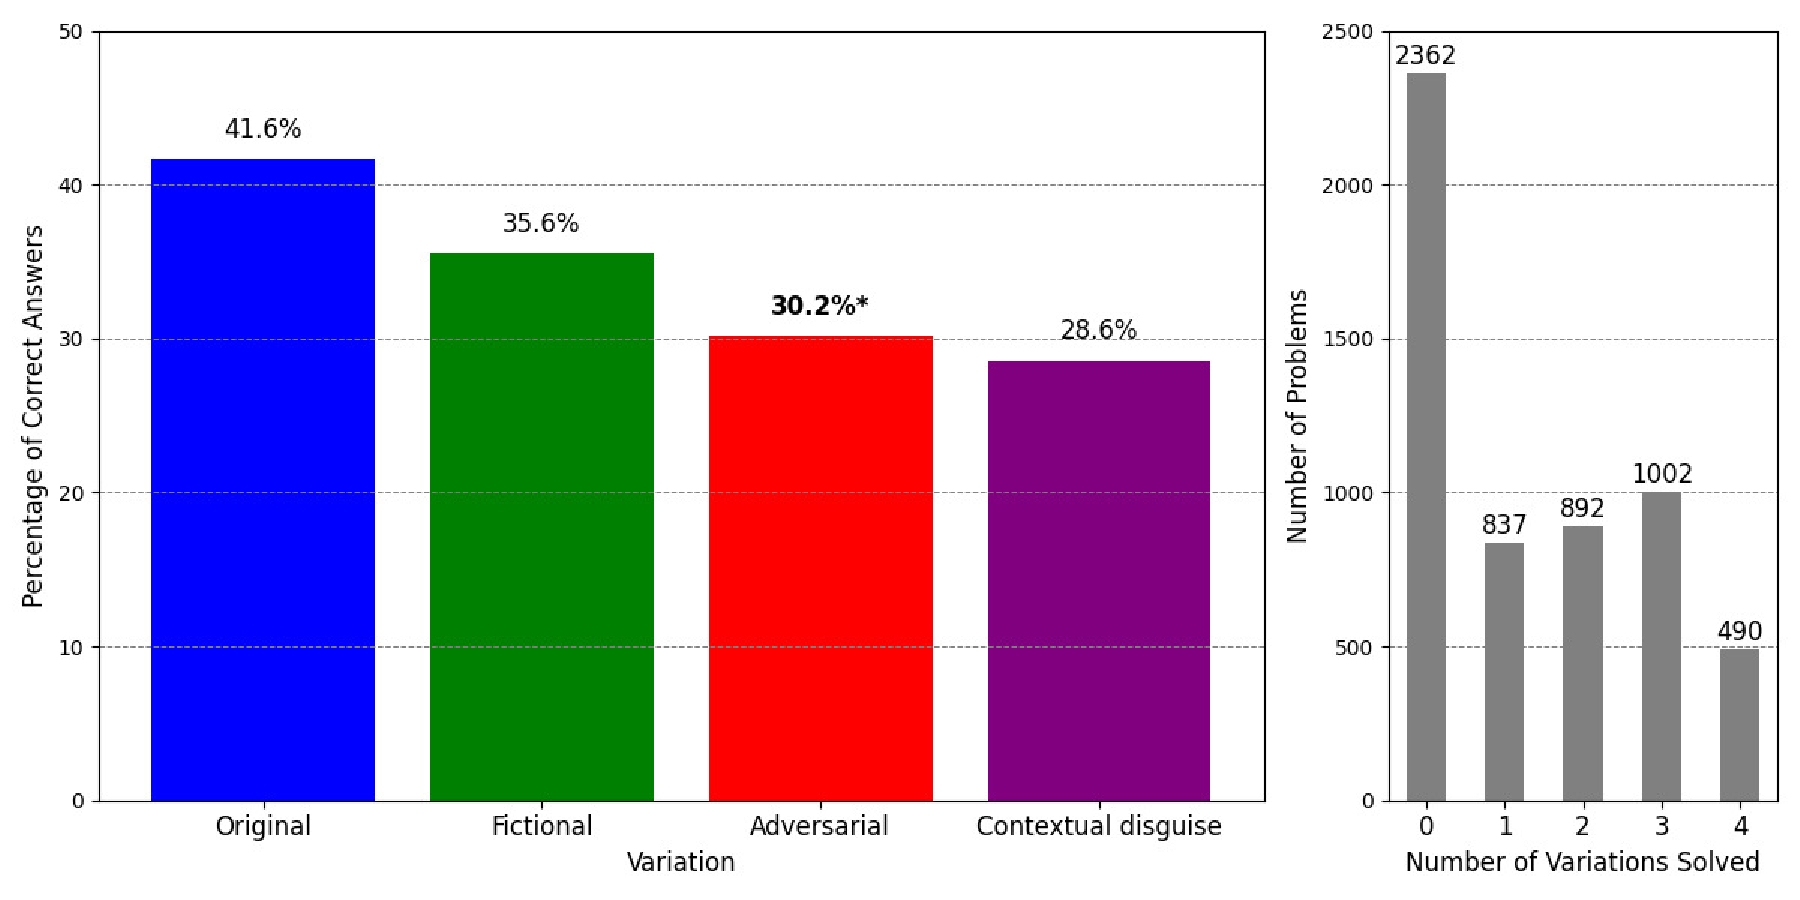
\includegraphics[width=0.9\textwidth]{synthetic_5583_avg.pdf}
    \caption{Ліворуч зображено частоту правильно розв'язаних варіацій до задач: оригінальна задача (блакитний), художня (зелений), суперечлива (червоний), прихована (фіолетовий). Праворуч зображено кількість правильно розв'язаних варіацій для кожної задачі. `*' вказує, що різниця у варіаціях була значуща ($p < .05$).}
    \label{fig:versions}
\end{figure}

\begin{figure}[ht]
    \centering
    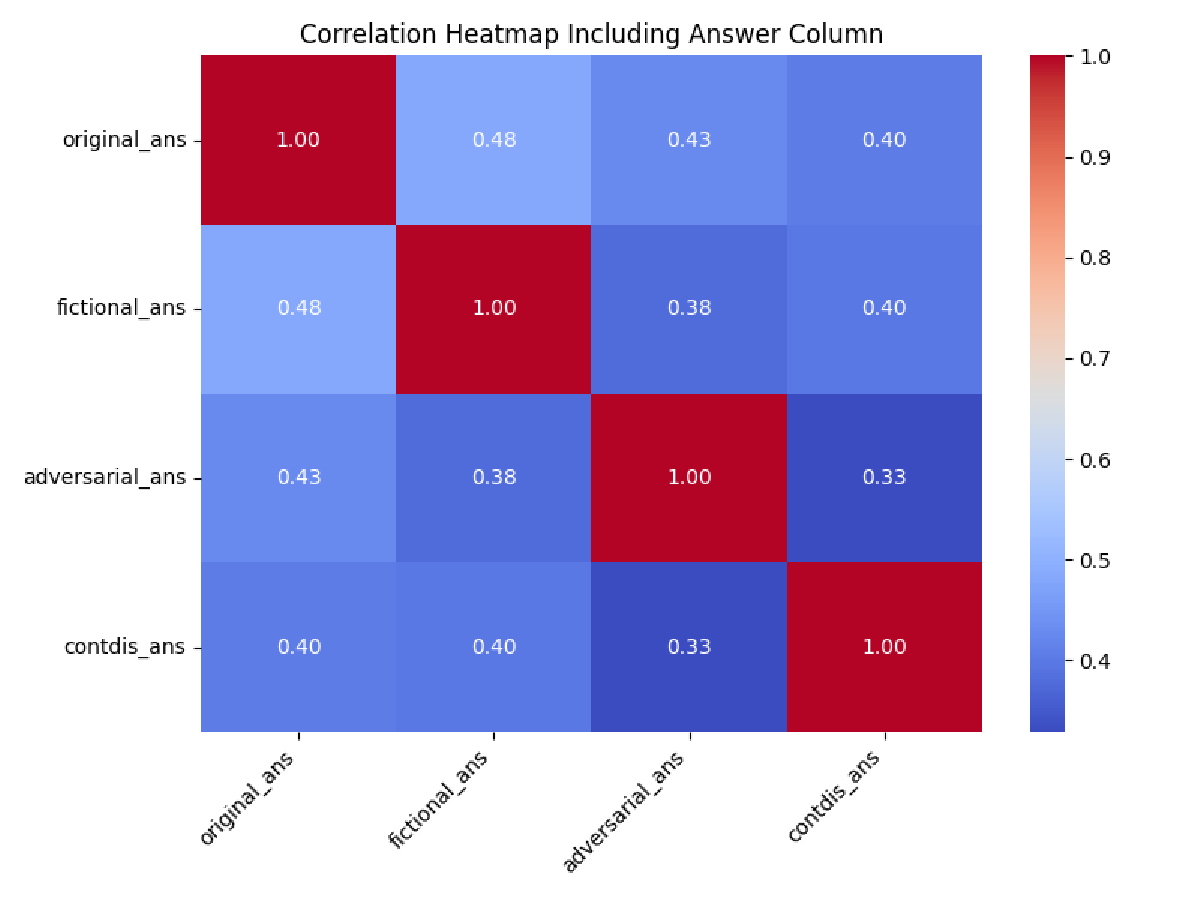
\includegraphics[width=0.9\textwidth]{synthetic_5583_corr.pdf}
    \caption{Коефіцієнт кореляції варіацій задач.}
    \label{fig:corr}
\end{figure}

Незважаючи на найбільшу середню довжину формулювання художньої варіації задачі ($len_{fictional}=651$ символів), дана варіація продемонструвала найкращі результати серед згенерованих синтетичний варіацій (35.6\%). Результати перевірки значущості показали, що порівняння між оригінальними розв'язками та розв'язками надлишкової варіації (\texttt{adversarial\_ans}) були значущими, у той час як порівняння з іншими варіаціями не виявили значних відмінностей. З наведених результатів також можна бачити, що у випадках, коли задача була розв'язана правильно, це було відбувалося у 3 з 4 варіацій задач (у 1002 випадках із 5583 протестованих задач), що також вказує на те, що принаймні рівно одна варіація у більшості випадків була не розв'язана моделлю.

Окремо слід зазначити, що під час проведення експериментально частини на 1000 тестових задачах, статистично значущою була різниця між оригінальними відповідями та відповідями надлишкової варіації (\texttt{contdis\_ans}) -- можлива ознака того, що збільшення набору даних призвело до покращення результатів оцінювання.

Для кореляційного аналізу було розглянуто результати різних варіацій, щоб побачити наскільки часто варіації однієї і тієї ж самої задачі розв'язувалися або не розв'язувалися моделлю правильно. На рисунку~\ref{fig:corr} видно слабку кореляцію між представленими варіаціями (між .33 і .48), що свідчить про те, що варіації не сильно пов'язані між собою. Це також свідчить про те, що процес генерації даних охоплює різноманітність, зберігаючи при цьому однакову результативність у кількості наданих правильних відповідей.

\subsection{Показник варіаційної узгодженості}

Для якості згенерованих моделей варіацій задач та їх впливу на точність розв'язань -- запропоновано нову метрику \textit{показник варіаційної узгодженості} (Variation Consistency Score). Ця метрика поєднує точність моделі та рівень кореляції між варіаціями задач, що дозволяє оцінити здатність моделей генерувати різноманітні, але точні із точки зору збереження сутності задачі тексти \cite{nikolaiev2025synth}.

Ця метрика поєднує в собі два ключові компоненти:

\begin{enumerate}
    \item \textbf{Частота правильних розв’язків (Solution rate)}: Відсоток правильно розв'язаних задач для заданої варіації моделлю.
    \item \textbf{Рівень кореляції варіацій (Correlation rate)}: Коефіцієнт кореляції між правильними відповідями та очікуваною відповіддю. Високий рівень кореляції свідчить про те, що варіації демонструють подібні результати та передають математичну основу задачі.
\end{enumerate}

Показник варіаційної узгодженості поєднує дані компоненти за допомогою середнього гармонійного значення (міри F1), забезпечуючи збалансовану оцінку, яка враховує точність роботи моделей та узгодженість варіації з оригінальною версією задачі. Даний показник обчислюється за наступною формулою:

\begin{equation}
\text{Variation Consistency Score} = \frac{2 \times (\text{Sol.rate} \times \text{Corr.rate})}{\text{Sol.rate} + \text{Corr.rate}}
\end{equation}

Показник варіаційної узгодженості акцентує увагу на ефективність роботи моделі: (i) оцінює наскільки модель є точною (відсоток правильно наданих відповідей по новій варіації задачі) і (ii) придатної до збереження математичної основи у новій варіації (висока кореляція між відповідями нової варіації та оригінальної) -- таким чином пропонуючи надійний показник для порівняння моделей у синтетичній генерації даних.

У таблиці \ref{tab:f1} наведено результати для варіацій задач, представлених у статті. Найвищу оцінку отримала художня варіація (.409) завдяки найвищій частоті правильності відповідей та високої кореляції з оригінальними даними.

\begin{figure}
    \centering
    \captionof{table}{Частота розв'язання (Sol.rate), коефіцієнт кореляції (Corr.rate) та показник узгодженості варіацій (Var.consist.)}
    \label{tab:f1}
    \begin{tabular}{|l|c|c|c|}
        \hline
        \textbf{Варіація} & \textbf{Sol.rate} & \textbf{Corr.rate} & \textbf{Var.consist.} \\
        \hline
        Художня & .356 & .482 & .409 \\
        Надлишкова & .302 & .428 & .354 \\
        Прихована & .286 & .404 & .335 \\
        \hline
    \end{tabular}
\end{figure}

%%%%%%%%%%%%%%%%%%%%%%%%%%%%%%%%%%%%%%%%%%%%%%%%%%%%%%%
\section{Аналіз результатів експерименту з участю експертів}

Наступний експеримент присвячено аналізу результатів експертів на наборі даних \emph{Combi-Puzzles}. Як згадувалося у підготовці експерименту у Розділі~\fullref{sec:human-experiment-set-up}, задля збереження репрезентативності експертів обиралися 5 учасників з найкращими результатами з кожної групи. Експерти певної групи отримували однаковий набір задач, проте працювали окремо один від одного.

Результати, представлені на Рисунку~\ref{fig:human_results}, свідчать, що експерти, середній вік яких становив 16 років, витратили в середньому 63 хвилини на розв’язання задач і у середньому отримали 70\% правильних розв'язків.

\begin{figure}
    \centering
    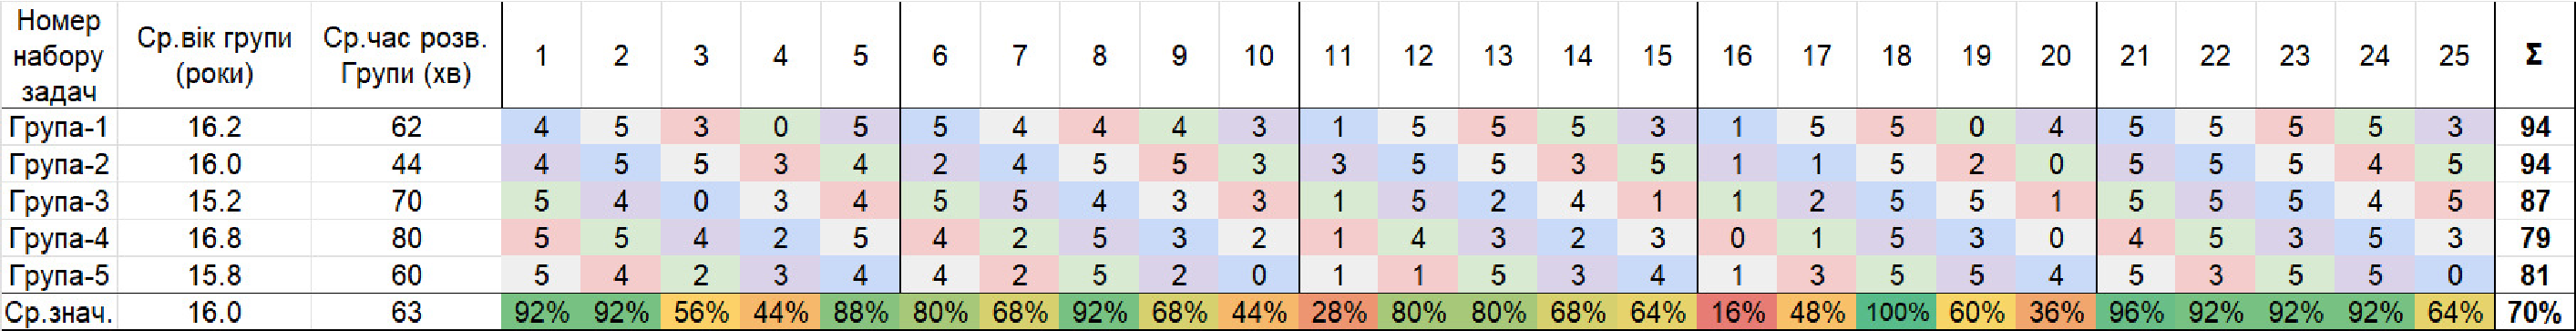
\includegraphics[width=1\textwidth]{data/human_results_top5.pdf}
    \caption{Результати 5 найкращих по кожній групі експертів на наборі задач Combi-Puzzles.}
    \label{fig:human_results}
\end{figure}

Загалом, усі експерти у своїх розв’язках забезпечили правильні рішення для кожної задачі щонайменше в одній з її варіацій. Проте, з Рисунку~\ref{fig:human_results} видно, що задачі 3, 4, 10, 11, 16, 17, 19 та 20 мають нижчі середні показники розв’язання (56\%, 44\%, 44\%, 28\%, 16\%, 48\%, 60\% та 36\% відповідно) порівняно з очікуваними 70\%.

У деяких випадках показник розв’язання був нижчим за очікуваний, що можна пояснити складністю певних задач. Наприклад, експерти надали лише кілька правильних розв’язків на задачі 11 та 16 (менше 30\% у всіх варіаціях), що може свідчити про їхню високу складність для розв’язання.

Для задач 4, 10, 16, 20 та 25 також спостерігалося, що жоден з експертів не зміг розв’язати задачу в одній або двох її варіаціях. Це може свідчити про те, що за певних змін умов задачі вони стають складними для розуміння навіть для експертів. Ці випадки будуть детальніше розглянуті у наступному підрозділі.

%%%%%%%%%%%%%%%%%%%%%%%%%%%%%%%%%%%%%%%%%%%%%%%%%%%%%%%
\section{Порівняння результатів роботи між моделями та експертами}

\begin{figure}
\centering
    \captionof{table}{Середні показники GPT-4 (без додаткової інструкції) та експертів за правильно розв’язаними задачами у різних умовах та загалом.}
    \begin{tabular}{|l|ccccc|c|}
        \hline
        Модель & Звич. & Матем. & Надлишк. & Парам. & Лінг. & Загал. \\
        \hline
        GPT-4 & .82 & .94 & .77 & .67 & .70 & .78 \\
        Експерти & .78 & .63 & .64 & .70 & .74 & .70 \\
        \hline
    \end{tabular}
    \label{tab:forms_human_v_model}
\end{figure}

У Таблиці~\ref{tab:forms_human_v_model} показано різницю в ефективності між експертами та ВММ за різними варіаціями задач і загалом. Із таблиці випливає, що найкраща модель (GPT-4) значно перевершує експертів у загальному показнику. Також спостерігається, що GPT-4 має високий результат у математичній формі задач (94\%), тоді як експерти досягли лише 63\%. Це може пояснюватися тим, що GPT-4 імовірно зустрічала подібні математичні тексти під час навчання.

Використання тесту Манна–Уїтні для порівняння середніх показників показало, що вплив математичної варіації є суттєвим ($p = .011 < .05$) порівняно з відсутністю математичної форми ($p = .281 > .05$). Для надлишкової варіації GPT-4 отримала вищий показник (77\%) порівняно з експертами (64\%), проте різниця не виявилася статистично значущою ($p=.185$). Надлишкова варіація створена додаванням нерелевантної інформації до звичайної постановки задачі, що, ймовірно, спричиняє більшу плутанину для експертів.

У випадку лінгвістичного заплутування різниця між моделями та експертами є набагато меншою (70\% для GPT-4 проти 74\% в експертів) і навіть трохи краща для останніх. Проте ця різниця не визнається статистично значущою ($p=.714$). Одна з гіпотез полягає в тому, що ефективність GPT-4 у лінгвістично заплутаній варіації знижується через більшу кількість тексту, що ускладнює виокремлення релевантної інформації.

Для параметризованої форми ефективність GPT-4 порівняно з експертами майже однакова (67\% проти 70\%), що може свідчити про недостатню точність моделі під час обчислень із більшим обсягом арифметики. У деяких випадках було відзначено, що попри правильні кроки обґрунтування GPT-4 могла генерувати неправильні ланцюги виразів, що призводило до хибних результатів.

З Таблиці~\ref{tab:forms_diff} видно, що результативність GPT-4 є чутливою до відмінностей у формулюваннях задач, які було задано п’ятьма формами у нашому наборі даних. Зокрема, було виявлено, що GPT-4 значно краще розв’язує комбінаторні задачі, подані в математичній формі (94\%), порівняно з надлишковими, лінгвістично заплутаними та параметризованими варіаціями (77\%, 70\% та 67\% відповідно). Це свідчить про певну нездатність моделі до узагальнення у міркуванні без додаткових етапів навчання моделей. Утім, дані висновки отримані на дослідження роботи моделей з набором даних Combi-Puzzles, які підтвердження у відповідному дослідженні.

Водночас, різниця у частоті надання правильних розв'язків експертами серед різних варіацій не є статистично значною. Це вказує на те, що здатність експертів до розв’язання комбінаторних задач не є залежною до модифікацій текстів задач.

На деяких варіаціях модель GPT-4 значно перевершує експертів, особливо у задачах із чітким формулюванням (математична варіація) і без додаткових лінгвістично-стилістичних маніпуляцій. Проте експерти виявляються більш гнучкими у розв’язанні задач з нестандартними умовами та можуть краще адаптуватися до модифікацій у формулюванні задач \cite{nikolaiev2024can}.

\section{Детальний аналіз окремих випадків задач}

\begin{figure}
    \centering
    \begin{subfigure}{\linewidth}
        \centering
        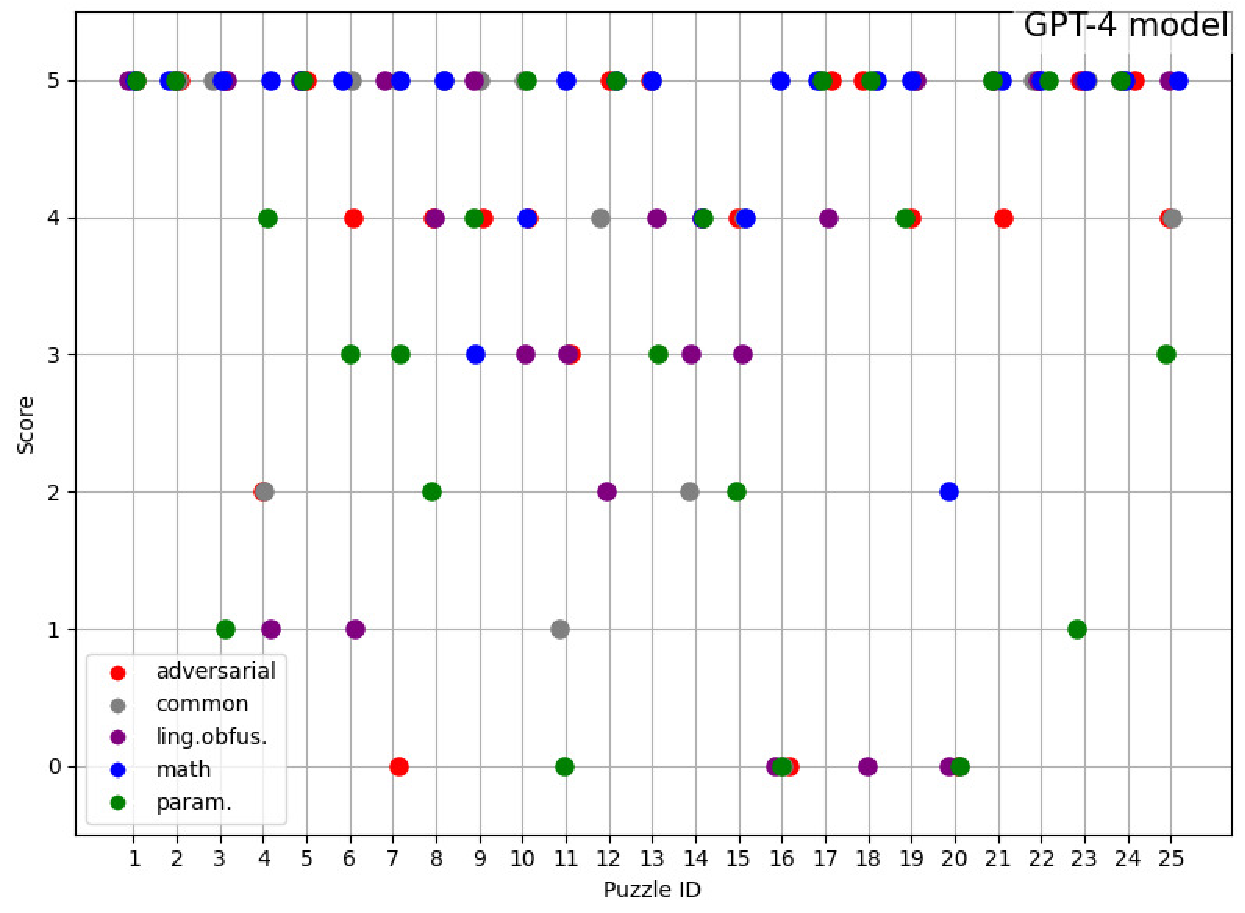
\includegraphics[width=0.75\linewidth]{data/Image-GPT-4.pdf}
        \caption{GPT-4}
        \label{fig:subimage_gpt4}
    \end{subfigure}
    \begin{subfigure}{\linewidth}
        \centering
        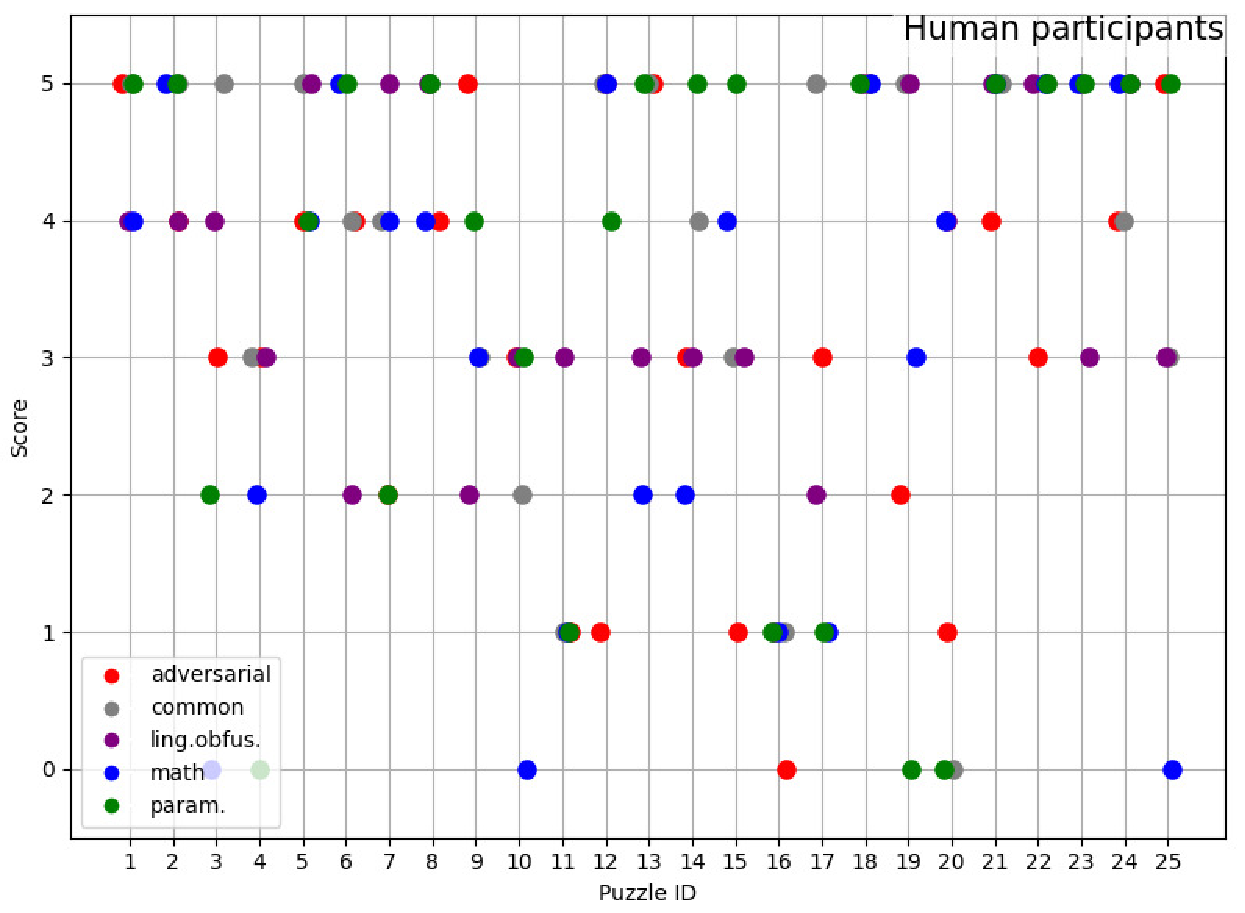
\includegraphics[width=0.75\linewidth]{data/Image-Humans.pdf}
        \caption{Експерти}
        \label{fig:subimage_humans}
    \end{subfigure}
    \caption{Індивідуальні бали за задачі та відсоток правильних розв’язків, представлені для GPT-4 та експертів.}
    \label{fig:humans_v_models_problems}
\end{figure}

Аналіз окремих задач надав можливість з’ясувати, які варіації задач були найскладнішими для експертів та ВММ. На Рисунку~\ref{fig:humans_v_models_problems} зображено кількість правильних розв’язків, наданих GPT-4 та експертами по кожній варіації задач у наборі \emph{Combi-Puzzles}. По осі X зазначено номер задачі, а по осі Y -- кількість правильних розв’язків. Результати тестування моделі GPT-4 формувалися на основі 5 запитів (кожен запит виконувався у окремій сесії), а результати тестування експертів -- з 5 учасників з найкращим результатом серед кожної групи.

З Рисунку~\ref{fig:humans_v_models_problems} видно, що кількість правильних розв’язків наданих експертами варіюється більше ніж кількість розв’язків від GPT-4. Модель має більш поляризовану тенденцію: якщо GPT-4 здатна розв’язати відповідну задачу у запропонованій варіації, вона зберігає цей результат на решті запитів. Натомість здатність експертів розв’язати задачі у різних варіаціях залежить від індивідуальних особливостей кожного учасника та їхнього досвіду у комбінаториці.

Також помітно, що в деяких випадках жоден з запитів моделі GPT-4 та експерти не надали жодного правильного розв’язку для окремих задач. Зокрема, задачі p4/param, p10/math та p25/math були розв’язані GPT-4 у 4, 5 та 5 випадках відповідно, тоді як експерти не дали жодного правильного розв’язку. Аналогічно задачі p18/ling.obfus та p20/ling.obfus були розв’язані експертами у 5 та 4 випадках відповідно, тоді як GPT-4 не надала жодного правильного розв’язку. Повні формулювання цих задач наведено у таблиці~\ref{tab:problems-poorly-solved}. Кожну задачу та її варіацію у таблиці задано ідентифікатором у вигляді ProblemID/variation. У відповідних стовпчиках таблиці зазначено кількість разів, коли задачу було правильно розв'язано (1) моделлю GPT-4 та (2) експертами. Тексти задач наведені українською мовою, якою проводилося експериментальна частина з людьми. Моделі під час експериментування працювали з англійськими текстами задач. Мови були обрані відповідно до того, на яких моделі мали більше попереднього тренування, а учасники -- математичного шкільного досвіду.

% \renewcommand{\arraystretch}{0.8} % change the interval between lines
\begin{figure}[!h]
    \centering
    \small
    \captionof{table}{Деякі приклади задач з найгіршими результатами розв'язання серед моделі GPT-4 (а) та експертів (б).}
    \label{tab:problems-poorly-solved}
    \begin{tabular}{|p{14cm}|c|c|}
        \hline
        \textbf{ID задачі та Умова} & \textbf{а} & \textbf{б} \\
        \hline
        \textbf{p4/param:} У кінотеатрі черга на фільм. Квиток коштує 5 фунтів. 5 людей мають банкноту у 10 фунтів кожна, і ще 5 людей мають банкноту у 5 фунтів кожна. На початку касир немає решти. Скільки існує різних способів формування черги, щоб кожен міг купити квиток? & 4 & 0 \\
        \hline
        \textbf{p10/math:} У скрині є 3 кулі, які пронумеровані від 1 до 3. Ви дістаєте кулі 9 разів одну за одною, кожного разу повертаючи кулю назад до скрині. Скільки різних можливих наборів куль ви можете отримати? & 5 & 0 \\
        \hline
        \textbf{p18/ling.obfus:} Лицар, який живе у місті Ґрінфілдс, планує брати участь на щорічних лицарських змаганнях. По-перше, він повинен доїхати до містечка Понівіль, де отримає свого благородного скакуна. Є 3 дороги між Ґрінфілдсом і Понівілем. У нього є вибір з 7 коней у Понівилі. Після цього він повинен поїхати у місто Садделфорд та обрати новий блискучий та комфортний садунок. Є 5 доріг між Понівілем і Садделфордом. Скільки існує шляхів, щоб подорожувати з Ґрінфілдса до Садделфорда через Понівіль? & 0 & 5 \\
        \hline
        \textbf{p20/ling.obfus:} Ви керуєте двома островами та церемоніальним човном, і ваша робота полягає у тому, щоб зробити кілька підготувань до важливого фестивалю. На кожному острові знаходять найвище дерево, яке потім вирізають у тотем, щоб розмістити на пляжі. Як тільки зрубають одне з двох дерев, на материк надсилається телеграма разом з датою та часом. Коли один з двох тотемів встановлено на пляжі, надсилається інша телеграма. Також вам потрібно переконатися, що церемоніальний човен буде прикрашено. Коли й ця робота буде завершена, надсилається ще одна телеграма. У вас є працівники на кожному острові та човні. Ви не знаєте, скільки часу займає кожна робота. Наприкінці підготувань ви дивитесь на порядок отриманих телеграм. Скільки існує різних послідовностей? & 0 & 4 \\
        \hline
        \textbf{p25/math:} У скрині знаходиться 25 куль білого кольору, які пронумеровані від 1 до 25, та 25 куль чорного кольору, які пронумеровані від 1 до 25. Ви дістаєте по одній 25 куль, не повертаючи їх назад до скрині. Щоразу коли ви дістаєте кулю з номером N певного кольору, куля з таким самим номером іншого кольору зникає зі скрині. Скільки різних послідовностей куль існує, які містять максимум 3 чорних кулі? & 5 & 0 \\
        \hline
    \end{tabular}
\end{figure}

У задачі p25/math комбінаторний розв’язок містить окремі підзадачі з нулем, однією та кількома чорними кулями, після чого застосовується правило суми: \(C(25, 0) + C(25, 1) + C(25, 2) + C(25, 3) = \sum_{i=0}^{3} C(25, i)\). Аналіз розв’язків GPT-4 свідчить, що модель правильно поділила задачу на підзадачі, розв’язала їх і підсумувала результати. Дана задача є однією з найскладніших у наборі даних, її математичну варіацію не розв’язав жоден з експертів.

Також GPT-4 продемонструвала кращий результат у задачі p10/math порівняно з експертами. Експерти не врахували, що шукається \textit{кількість різних наборів} куль, і надали розв’язок \(3^9\). Натомість GPT-4 правильно розпізнала умову й обрала відповідну комбінаторну формулу: \(C(11, 2) = 55\).

В окремих випадках модель GPT-4 виявляла здатність ідентифікувати математичні концепції у задачах та застосовувати їх для розв’язання більших складних випадків параметризованої варіації задач. Наприклад, у задачі p4/param GPT-4 розпізнала послідовність чисел Каталана і відразу використала формулу \(C_n = \frac{(2n)!}{(n + 1)!n!}\), що дозволило отримати правильний розв'язок.

Водночас GPT-4 мала певні труднощі з розв’язанням варіацій лінгвістичного заплутування, які вважаються одними з найпростіших у наборі даних: задачі p18/ling.obfus та p20/ling.obfus були успішно розв’язані експертами, тоді як GPT-4 не надала жодного правильного розв’язку. Це свідчить про те, що додавання нерелевантної інформації або зміна стилю викладу задачі ускладнюють для моделі відокремлення суттєвої інформації задачі.

Прикладом додаткових умов є задача: ``Визначте кількість різних способів, якими тура може переміститися з початкової до кінцевої позиції на шаховій дошці 3×3, \textit{не проходячи через середню клітинку.}''. Усі три конфігурації моделі LLaMA 3.1 (з урахуванням 8, 70 та 405 млрд. параметрів) успішно розв’язали початкову версію задачі, надавши правильний розв’язок. З  рис.~\ref{fig:prob_constraints} можна бачити, що у випадку з додатковим обмеженням про заборону використання середньої клітинки дошки, модель неправильно порахувала кількість можливих шляхів. Натомість експерти не зазнали подібних труднощів, правильно зазначивши, що кількість правильних шляхів дорівнює 2.

\begin{figure}[h]
    \centering
    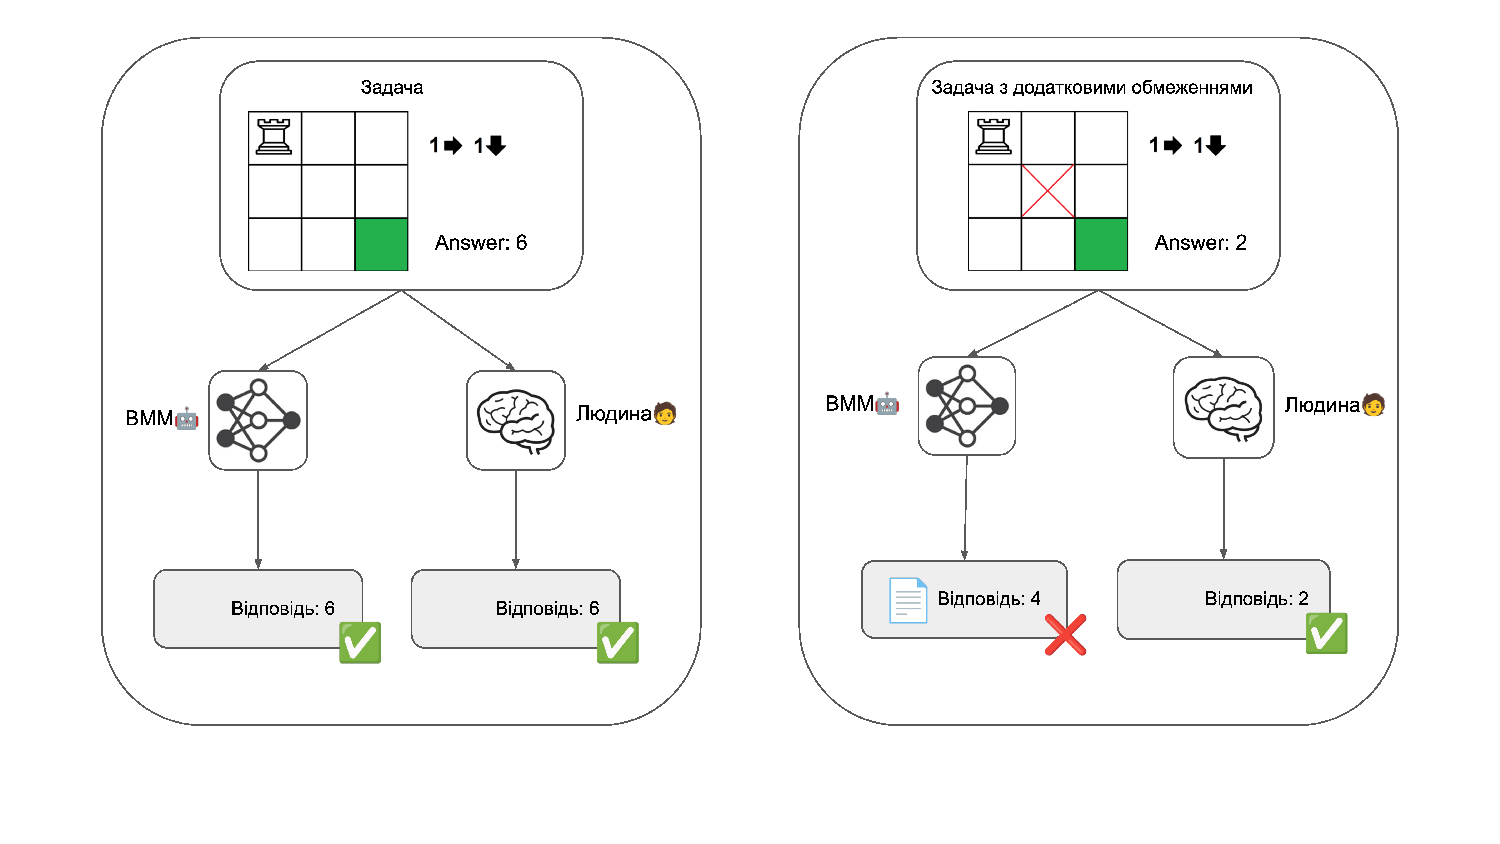
\includegraphics[width=1\textwidth]{prob_constraints.pdf}
    \caption{LLaMA 3.1 і експерти, що розв’язують комбінаторну задачу у двох умовах: звичайну версію та з додатковими обмеженнями.}
    \label{fig:prob_constraints}
\end{figure}

Таким чином, виявлено що моделі не завжди здатні розв'язувати задачі через неправильне розуміння умов або неможливість врахувати усі можливі варіанти відповіді. Наприклад, мовні моделі закономірно пропускають ключові деталі або не враховувати додаткові обмеження, що свідчить про потребу подальшого вдосконалення самоаналізу на необхідності внутрішнього міркування моделей.

\section{Висновки та подальші дослідження}

\paragraph{Вплив математичних роздiлiв на ефективність моделей при розв'язанні задач.}
Дослідження демонструє застосування передових мовних моделей для оцінки ефективності розв’язання задач у різних математичних розділах. Під час роботи з набором даних NuminaMath-TIR було виявлено значні відмінності у ефективності роботи моделей у генерації розв'язків між виділеними математичними розділами: алгебра, геометрія, теорія чисел та комбінаторика. Результати підтверджують статистично значущу залежність між математичними розділом та частотою правильних розв’язків. Найбільш складною темою виявилася комбінаторика, на якій протестовані моделі продемонстрували найнижчі результати.

Проведений аналіз засвідчує послідовні закономірності поведінки протестованих моделей: розділ алгебри зазвичай дає найвищі результати для всіх моделей, що свідчить про високу здатність працювати з формальними текстами. Водночас комбінаторика стабільно виявляється найскладнішою для пошуку правильних розв’язань у більшості випадків. Врахування особливостей походження математичних задач є важливим для подальшого покращення роботи моделей при розв'язанні математичних задач. Зокрема, важливим є підготовка та класифікація навчальних наборів даних орієнтованих для виправлення в ефективності моделей за різноманітними розділами.

Хоча усі відмінності в ефективності моделей між розділами були значущими, спостерігалося, що деякі моделі, зокрема GPT-4o-mini і Llama-3.1-8B-Instruct, виявляють більшу чутливість до відповідних розділів задач ($\chi^2_{\text{}}>180$). Для моделей Mathstral-7B та Qwen2.5-Math-7B характерні більш стабільні показники ефективності в розділах задач ($\chi^2_{\text{}}<150$). Це підкреслює важливість використання таких технік, як інтегроване розуміння з інструментами ToRA, задля отримання більш стабільних результатів моделей по різних математичних розділах задач. Про це також свідчать результати ВММ Qwen2.5-Math-7B, яка згідно опису має інтегрований ToRA, але незважаючи на відносно невеликий розмір моделі, показала вищу загальну ефективність у всіх розділах задач.

Ці результати наголошують на важливості врахування специфіки розділів різноманітних математичних задач для подальшого дослідження моделей у галузі обробки математичних даних. Це може сприяти створенню адаптивних систем навчання, здатних ефективно сприймати тонкощі різних математичних розділів.

\paragraph{Висновки дослідження з набором даних Combi-Puzzles}
Було запроваджено набір даних \emph{Combi-Puzzles} для оцінки здатності ВММ до міркування у комбінаторних задачах та методологію для створення наборів даних для цього завдання. За підсумками результатів експериментів GPT-4 продемонструвала найбільш високу роботу з математичними комбінаторними задачами серед протестованих ВММ. Зокрема, було встановлено, що модель у середньому повертає більшість кількість правильних розв'язків у порівнянні з учасниками з олімпіадним досвідом.

Результати свідчать про те, що здатність GPT-4 до міркувань вища, коли комбінаторні задачі представлені у формально-математичному стилі (математична варіація, 94\%). Однак також було установлено, що у наведеному наборі даних ефективність GPT-4 значно погіршується, коли у текстах задачі вводиться зайва інформація (надлишкова варіація, 77\%), коли умова задачі представлена у незнайомому наративному стилі (лінгвістичне заплутування, 70\%), а також при зміни параметрів задачі (параметризована варіація, 67\%). Незважаючи на гірші середні показники, учасники у дослідженні мали різні  надання правильних точності на досліджуваних варіаціях задач, не було виявлено залежностей між частотою надання правильних розв'язків та варіаціями задач.

\paragraph{Вдосконалені методів генерації синтетичних комбінаторних задач}
У роботі було проведено дослідження використання нейромережевих методів відбору та генерації синтетичних варіацій комбінаторних задач із залученням сучасної великої мовної моделі GPT-4o-mini. За допомогою запропонованого методу було відібрано дані та згенеровано синтетичні варіації, зберігаючи основний зміст математичних задач. Це дозволило оцінити здатність моделей до узагальнення міркування та слідування заданим інструкціям. Знайти приклади згенерованих задач можна у Додатку~\fullref{sec:problems-synthetic}.

Статистичний аналіз за допомогою тестів на перестановку показав, що модель не виявляє суттєвих відмінностей у розв'язанні введених варіацій задач порівняно з оригінальною, за винятком \emph{прихованої варіації}, яка отримала найнижчі оцінки. Водночас кореляційний аналіз варіацій, згенерованих нейромережевими методами, показав, що задачі мають низький рівень взаємозв'язку між собою. Знижений ризик повторюваності означає, що кожна варіація робить унікальний внесок у процес генерації текстів.

Окрім цього, для оцінювання здатності моделі до узагальнення було введено нову метрику -- \emph{Показник варіаційної узгодженості}, який поєднує частоту правильно наданих розв'язків задач та їхньою відповідністю оригінальним текстам. За результатами експериментування, незважаючи на найбільший розмір оброблених текстів, \emph{художня варіація} зберегла найвищу оцінку якості. Дані результати свідчать про те, що модель здатна генерувати унікальні та точні математичні дані, зберігаючи їхню математичну основу.

У майбутніх дослідженнях підкреслюється важливість підвищення адаптивності моделей шляхом вивчення вдосконалених методів навчання, які покращують обробку різноманітних текстових маніпуляцій. Це може бути досягнуто шляхом впровадження стратегій тренування моделей та нейро-символічних систем, а також використання різноманітних навчальних наборів даних. Зусилля в цьому напрямку можуть призвести до покращення загальної здатності моделей до узагальнення та підвищення їхньої стійкості в задачах математичного міркування.

\paragraph{Обмеження ВММ та напрямки подальших розробок}
Попри значущість отриманих результатів, дослідження має певні обмеження. Було продемонстровано, що мовні моделі виявляють високу чутливість до змін у формулюванні задач, що знижує точність розв'язань при введенні зайвої інформації або лінгвістичних модифікацій.

Складність комбінаторних задач та їх математичний підтекст іноді перевищують здатності моделей до адекватного міркування, що потребує інтеграції формальних методів, яку можна досягнути за рахунок розробки автоматизованих систем перевірки й формалізації синтетичних даних для забезпечення більш стабільної якості генерованих результатів.

Подальші дослідження можуть бути зосереджені на розробці модифікованих архітектур великих мовних моделей, стійкіших до стилістичних варіацій та надлишкової інформації. Такі архітектури мають передбачати інтеграцію формальних методів міркування й символьних обчислень з ВММ для підвищення точності та послідовності математичних розв'язань.

Іншим напрямком для поліпшення існуючих методів за рахунок отриманих результатів є розширенні підходів генерації синтетичних даних, з метою охоплення ширшого спектру математичних задач різних математичних розділів.

Не можна також забувати про важливість етичних аспектів використання штучного інтелекту в освіті та наукових дослідженнях, які сприяють подальшому вдосконаленню автоматизованих освітніх систем.

\paragraph{Практичне значення та перспективи використання отриманих результатів}
Практичне значення проведеного дослідження полягає в наступному:
\begin{itemize}
    \item Розроблені методи синтезу даних та генерації комбінаторних задач можуть бути використані для покращення адаптивних освітніх систем, що підтримують автоматизований процес навчання та оцінки учнів.
    \item Запропонована методологія формалізації математичних текстів дозволяє оптимізувати процес переведення задач з природної мови у формальні математичні вирази, що має важливе значення для розвитку автоматизованих систем доведень.
    \item Використання нової метрики варіаційної узгодженості дає можливість здійснювати більш глибокий аналіз якості генерованих даних, що може стати основою для подальших досліджень та комерційних застосувань у сфері штучного інтелекту.
    \item Результати експериментального дослідження сприяють побудові міцного містка між можливостями ВММ та практичними потребами математичної освіти та наукових розробок.
\end{itemize}

Таким чином, було проведено комплексний аналіз якості науково-методичного апарату, що підтверджує доцільність впровадження запропонованих кроків з метою покращення алгоритмів генерації розв’язань і синтезу даних математичних комбінаторних задач. Дані результати мають важливе значення для подальших досліджень за напрямком розвитку моделей у математичних задачах і практичного застосування мовний моделей у освітньо-практичних цілях.
